\chapter{Liveness \Author{B. Boissinot \andAuthor F. Rastello}}
\label{chapter:ssa_tells_nothing_of_liveness}
\inputpath{part3}{ssa_tells_nothing_of_liveness}
\inputprogress
\newcommand{\name}[1]{#1}
\newcommand{\firm}{\name{LibFirm}}
\newcommand{\lao}{\name{LAO}}
\newcommand{\stm}{\name{STMicroelectronics}}
\newcommand{\Nat}{\mathbb{N}}
\newcommand{\void}[1]{ }
\newcommand{\lstart}{\textrm{start}}
\newcommand{\paper}{paper\xspace}
\newcommand{\vundef}{\Box}
\newcommand{\domzone}[1]{\mathit{dom}({#1})}
\newcommand{\sdomzone}[1]{\mathit{sdom}({#1})}
\newcommand{\prenum}[1]{\mathit{prenum}({#1})}
\newcommand{\back}[1]{\mathcal{B}_{#1}}
\newcommand{\lb}[1]{\mathbf{#1}}
\newcommand{\ldef}[1]{\mathit{def}(\var{#1})}
\newcommand{\luse}[1]{\mathit{uses}(\var{#1})}
\newcommand{\reach}[2]{{#1}\rightarrow {#2}}
\newcommand{\redreach}[2]{{#1}\rightharpoondown {#2}}
\newcommand{\red}[1]{\widetilde{#1}}
\newcommand{\BEsrc}{V^\otimes}
\newcommand{\BEtgt}{V^\odot}
\newcommand{\BE}{E^\uparrow}
\newcommand{\Tqa}{T_{(q,\var a)}}
\newcommand{\alain}[1]{{\color{red} #1}}
\newcommand{\reduced}{forward}
\newcommand{\Reduced}{Forward}
\def\Live{\textrm{Live}}
\def\LiveOut{\textrm{LiveOut}}
\def\LiveIn{\textrm{LiveIn}}
\def\PhiKill{\textrm{PhiDefs}}
\def\PhiUses{\textrm{PhiUses}}
\def\Kill{\textrm{Defs}}
\def\Exit{\textrm{Exit}}
\def\Entry{\textrm{Entry}}
\def\UpExp{\textrm{UpwardExposed}}
\def\cfgsuccs{\textrm{CFG\_succs}}
\def\union{\cup}
\def\Def{\textrm{def}}
\def\phidefedge{\texttt{phidef\_edge}}
\def\phiuseedge{\texttt{phiuse\_edge}}
\def\top{\textrm{top}}
\def\push{\textrm{push}}
\def\pop{\textrm{pop}}

\section{Introduction}
This chapter illustrates the use of strict SSA properties\index{strict SSA form} to simplify and accelerate \emph{liveness analysis}, which determines for all variables the set of program points where they are \emph{live}, i.e., their values are potentially used by subsequent operations.
Liveness information is essential to solve storage assignment problems, eliminate redundancies, and perform code motion.
For instance, optimizations like software pipelining, trace scheduling, register-sensitive redundancy elimination, if-conversion, as well as register allocation heavily rely on liveness information.

% What is the problem

Traditionally, liveness information is obtained by data-flow analysis\index{data-)flow analysis}:
liveness sets are computed for all basic blocks and variables simultaneously by solving a set of data-flow equations.
These equations are usually solved by an iterative algorithm, propagating information backwards through the control-flow graph (CFG) until a fixed point is reached and the liveness sets stabilize.
The number of iterations depends on the control-flow structure of the considered program, more precisely on the structure of its loops.

% What is our main result. I think this is simple enough so that is can be put it in the introduction
In this chapter, we show that, for strict SSA-form programs, the live-range of a variable has nice properties that can be expressed in terms of loop nesting forest of the CFG and its corresponding directed acyclic graph, the \emph{forward-CFG}\index{forward control-flow graph}.
Informally speaking, and restricted to reducible CFGs, those properties for a variable $v$ are:
\begin{itemize}
\item
	$v$ is live at a program point~$q$ if and only if $v$ is live at the entry~$h$ of the largest loop/basic block (highest node in the loop nesting forest\index{loop nesting forest}) that contains~$q$ but not the definition of~$v$.
\item
	$v$ is live at~$h$ if and only if there is a path in the forward-CFG from~$h$ to a use of~$v$ that does not contain the definition.
\end{itemize}

% What is our solution for liveness sets computation

A direct consequence of this property is the possible design of a data-flow algorithm that computes liveness sets \emph{without the requirement of any iteration} to reach a fixed point:
at most two passes over the CFG are necessary.
The first pass, very similar to traditional data-flow analysis, computes partial liveness sets by traversing the forward-CFG backwards.
The second pass refines the partial liveness sets and computes the final solution by propagating forward along the loop nesting forest.
For the sake of clarity, we first present the algorithm for reducible CFGs.
Irreducible CFGs can be handled with a slight variation of the algorithm, with no need to modify the CFG itself.

% Other var-by-var etc approaches for liveness sets computation
Another approach to liveness analysis more closely follows the classical definition of liveness:
a variable is live at a program point~$q$ if~$q$ belongs to a path of the CFG leading from a definition of that variable to one of its uses without passing through another definition of the same variable.
Therefore, the live-range of a variable can be computed using a backward traversal starting on its uses and stopping when reaching its definition (unique under SSA).

% Our liveness check solution
One application of the properties of live-ranges under strict SSA-form is the design of an extremely simple liveness check algorithm.
In contrast to classical data-flow analyses, liveness check does not provide the set of variables live at a block, but its characteristic function.
Liveness check provides a query system to answer questions such as ``Is variable~$v$ live at location~$q$?''
Its main features are:
\begin{compactenum}
\item
	The algorithm itself consists of two parts, a \emph{pre-computation} part, and an \emph{online} part executed at each liveness query.
	It is not based on setting up and subsequently solving data-flow equations;
\item
	The pre-computation is \emph{independent of variables,} it only depends on the structure of the control-flow graph;
	Hence, pre-computed information \emph{remains valid} upon adding or removing variables or their uses;
\item
	An actual query uses the def-use chain of the variable in question and determines the answer essentially by testing membership in pre-computed sets of basic blocks.
\end{compactenum}

% Layout
We will first need to repeat basic definitions relevant in our context and provide the theoretical foundations in the next section, before presenting multiple algorithms to compute liveness sets: The two-pass data-flow algorithm in Section~\ref{sec:data-flow} and the algorithms based on path-exploration in Section~\ref{sec:path-explore}.
We finally present the liveness check algorithm last, in Section~\ref{sec:live-check}.
%% TODO: improve this introduction paragraph by adding some information, or just remove it.

\section{Definitions}
Liveness\index{liveness} is a property relating program points to sets of variables which are considered to be \emph{live} at these program points.
Intuitively, a variable is considered live at a given program point when its value will be used in the future of any dynamic execution.
Statically, liveness can be approximated by following paths backwards on the control-flow graph, connecting the uses of a given variable to its definitions---or, in the case of SSA forms, to its unique definition.
The variable is said to be \emph{live} at all program points along these paths.
For a CFG node~$q$, representing an instruction or a basic block, a variable $\var{v}$ is \emph{live-in} at~$q$ if there is a path, not containing the definition of $\var{v}$, from~$q$ to a node where $\var{v}$ is used (including $q$ itself).
It is \emph{live-out} at~$q$ if it is live-in at some successor of~$q$.

The computation of live-in and live-out sets at the entry and the exit of basic blocks is usually termed \emph{liveness analysis}.
It is indeed sufficient to consider only these sets at basic block boundaries since liveness within a basic block is trivial to recompute from its live-out set with a backward traversal of the block.
\emph{Live-ranges}\index{live-range} are closely related to liveness.
Instead of associating program points with sets of live variables, the live-range of a variable specifies the set of program points where that variable is live.
Live-ranges of programs under strict SSA form exhibit certain useful properties (see Chapter~\ref{chapter:properties_and_flavours}), some of which can be exploited for register allocation (see Chapter~\ref{chapter:register_allocation}).

The special behavior of $\phi$-functions often causes confusion on where exactly its operands are actually used and defined.
For a regular operation, variables are used and defined where the operation takes place.
However, the semantics\index{liveness!\phifun} of \phifuns\ (and in particular the actual place of \phiuses) should be defined carefully, especially when dealing with SSA destruction.
In algorithms for SSA destruction (see Chapter~\ref{chapter:alternative_ssa_destruction_algorithm}), a use in a \phifun is considered live somewhere inside the corresponding predecessor block, but, depending on the algorithm and, in particular, the way copies are inserted, it may or may not be considered as live-out for that predecessor block.
Similarly, the definition of a \phifun is always considered to be at the beginning of the block, but, depending on the algorithm, it may or may not be marked as live-in for the block.
%These subtleties need to be taken into account when building liveness sets.
To make the description of algorithms easier, we follow the same definition as the one used in Chapter~\ref{chap:alternative_ssa_destruction_algorithm}, Section~\ref{sec:alternative_ssa_destruction_algorithm:liveness}:
For a $\phi$-function $a_0 = \phi(a_1, \ldots, a_n)$ in block~$B_0$, where $a_i$ comes from block~$B_i$:
\begin{compactitem}
\item
	Its definition-operand is considered to be at the entry of $B_0$, in other words variable $a_0$ is live-in of $B_0$;
\item
	Its use-operands are at the exit of the corresponding predecessor basic blocks, in other words, variable $a_i$ is live-out of basic block $B_i$.
\end{compactitem}
This corresponds to placing a copy $a_0\gets a_i$ on each edge from $B_i$ to $B_0$.
The data-flow equations given hereafter and the presented algorithms follow the same semantics.
They require minor modifications when other $\phi$-semantics are desired.
%We will come back to these subtleties in Section~\ref{sec:correctnessdebase}.

\section{Data-Flow Approaches}
\label{sec:data-flow}

A well-known and frequently used approach to compute the live-in and live-out sets of basic blocks is backward data-flow analysis~\index{backward analysis} (see Chapter \ref{chapter:constant_propagation_is_easier}, Section~\ref{novillo:sec:preliminaries}).
The liveness sets are given by a set of equations that relate \emph{upward-exposed} uses and definitions to live-in and live-out sets.
We say a use is \emph{upward-exposed} in a block when there is no local definition preceding it, i.e., the live-range ``escapes'' the block at the top.

The sets of upward-exposed uses and definitions do not change during liveness analysis and can thus be pre-computed.
%
In the following equations, we denote $\PhiKill(B)$ the variables defined by \phifuns at the entry of block~$B$ and by $\PhiUses(B)$ the set of variables used in a \phifun at the entry of a successor of the block~$B$.

\begin{eqnarray*}
	\LiveIn(B) & = & \PhiKill(B) \cup \UpExp(B) \cup \,(\LiveOut(B)\setminus \Kill(B)) \\
	\LiveOut(B)& = &
	\textstyle \bigcup_{S \in \textrm{succs}(B)} (\LiveIn(S) \setminus
	\PhiKill(S)) \cup\, \PhiUses(B)
\end{eqnarray*}

Informally, the live-in of block $B$ are the variables defined in the 
\phifuns of $B$, those used in $B$ (and not defined in $B$), and those 
which are just ``passing through.'' On the other hand, the live-out are 
those that must be live for a successor $S$, i.e., either live-in of $S$ 
(but not defined in a \phifun of $S$) or used in a \phifun of $S$.


\subsection{Liveness Sets On Reducible Graphs}
\label{sec:forreducible}

Instead of computing a fixed point, we show that liveness information can be derived in two passes over the control-flow graph.
The first version of the algorithm requires the CFG to be reducible.
We then show that arbitrary control-flow graphs can be handled elegantly and with no additional cost, except for a cheap pre-processing step on the loop nesting forest.

The key properties of live-ranges under strict SSA form on a reducible CFG that 
we exploit for this purpose %and that we will formalize later on,
can be outlined as follow:
\begin{enumerate}
  \item
    Let~$q$ be a CFG node that does not contain the definition~$d$ of 
    a variable, and $h$ be the header of the maximal loop containing~$q$ 
    but not~$d$.
    If such a maximal loop does not exist, then let $h=q$.

    The variable is live-in at~$q$ if and only if there exists a forward path 
    from~$h$ to a use of the variable without going through the definition $d$.

  \item
    If a variable is live-in at the header of a loop then it is live at all 
    nodes inside the loop.
\end{enumerate}

As an example, consider the code of Figure~\ref{fig:examplecfg_run}. For $q=6$, the header of the largest loop containing $6$ but not the definition $d$ in $3$ is $h=5$. As there exists a forward path (down edges) from $3$ to $5$, variable $v$ is live-in at $5$. It is thus also live in all nodes inside the loop, in particular in node $6$. On the other hand, for $q=7$, the largest ``loop'' containing $7$ but not $3$ is $7$ itself. As there is no forward path from $7$ to any use (node $5$), $v$ is not live-in of $7$ (note that $v$ is not live-in of $2$ either).

Those two properties pave the way for describing the two steps that make up our liveness set algorithm:
\begin{compactenum}
\item
	A backward pass propagates partial liveness information upwards using a post-order traversal of the forward-CFG;
\item
	The partial liveness sets are then refined by traversing the loop nesting forest, propagating liveness from loop-headers down to all basic blocks within loops.
\end{compactenum}
Algorithm~\ref{alg:twopass} shows the necessary initialization and the high-level structure to compute liveness in two passes.

\begin{figure}[t]
   \begin{center}
       % 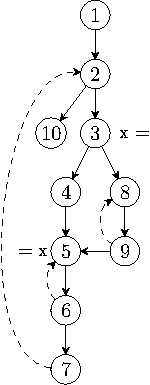
\includegraphics{examplecfg_run.pdf}
       \tikzfigure{examplecfg_run}
       \caption{An example of a reducible CFG. Forward CFG is represented using 
       full edges; back-edges are thickened. Backward pass on forward CFG sets 
     $v$ as live-in of node $5$, but not of node $2$. Forward pass on loop 
   nesting forest then sets $v$ as live at node $6$ but not at node $7$. }
       \label{fig:examplecfg_run}
   \end{center}
\end{figure}

\medskip
\begin{algorithm}[H]
    % \Func{Compute\_LiveSets\_SSA\_Reducible(CFG)}{
      \ForEach{basic block~$B$}{
          mark~$B$ as unprocessed\;
      }
      {DAG\_DFS}($r$) \Comment*{$r$ is the CFG root node}
      \ForEach{root node~$L$ of the loop nesting forest}{
        {LoopTree\_DFS}($L$)\;
      }
    % }
    \caption{Two-pass liveness analysis: reducible \@CFG.}
  \label{alg:twopass}
\end{algorithm}
\medskip

The post-order traversal is shown in Algorithm~\ref{alg:dag_dfs}, which performs a simple depth-first search and gives partial liveness sets to every basic block of the CFG.
The algorithm roughly corresponds to the pre-computation step of the traditional iterative data-flow analysis;
However, back-edges are not considered during the traversal.
Recalling the definition of liveness for \phifuns, $\PhiUses(B)$ denotes the set of variables live-out of basic block~$B$ due to uses by \phifuns in successors of $B$.
Similarly, $\PhiKill(B)$ denotes the set of variables defined by a \phifun in~$B$.

\medskip
\begin{algorithm}[H]
    \Func{DAG\_DFS(block~$B$)}{
      \ForEach{$S\in\textrm{succs}(B)$ such that $(B,S)$ is not a back-edge}{\label{alg:dag_dfs:loop_edge}
        \lIf{$S$ is unprocessed}{{DAG\_DFS}($S$)}\label{alg:dag_dfs:irreducible_dfs}
      }
      $\textit{Live}\ \gets \PhiUses(B)$\; \label{alg:dag_dfs:phi_use}
      \ForEach{$S\in\textrm{succs}(B)$ such that $(B,S)$ is not a back-edge}{
        $\textit{Live}\ \gets \textit{Live}\  \union \ (\LiveIn(S) \setminus \PhiKill(S))$ \label{alg:dag_dfs:phi_kill_minus}\label{alg:dag_dfs:irreducible}\;
      }
      $\LiveOut(B) \gets \textit{Live}$\;
      \ForEach{program point~$p$ in~$B$, backwards,}{
        remove variables defined at~$p$ from \textit{Live}\;
        add uses at~$p$ to \textit{Live}\;
      }
      $\LiveIn(B) \gets \textit{Live}\  \union\  \PhiKill(B)$ \label{alg:dag_dfs:phi_kill_union}\;
      mark~$B$ as processed\;
    }
  \caption{Partial liveness, with post-order traversal.}
  \label{alg:dag_dfs}
\end{algorithm}
\medskip

The next phase, which traverses the loop nesting forest, is shown in Algorithm~\ref{alg:loop_dfs}.
The live-in and live-out sets of all basic blocks within a loop are unified with the liveness sets of its loop-header.

\medskip
\begin{algorithm}[H]
    \Func{LoopTree\_DFS(node~$N$ of the loop nesting forest)}{
      \If{$N$ is a loop node}{
        $B_N \gets \textrm{Block}(N)$ \Comment*{The loop-header of~$N$}
        $\textit{LiveLoop} \ \gets \LiveIn(B_N) \setminus \PhiKill(B_N)$ \label{alg:loop_dfs:phi_kill_minus}\;
        \ForEach{$M \in \textrm{Children}(N)$}{
          $B_M \gets \textrm{Block}(M)$ \Comment*{Loop-header or block}
          $\LiveIn(B_M) \gets \LiveIn(B_M)\ \union\ \textit{LiveLoop}$\;
          $\LiveOut(B_M) \gets \LiveOut(B_M)\ \union\ \textit{LiveLoop}$\;
          {LoopTree\_DFS}($M$)\;
        }
      }
    }
  \caption{Propagate live variables within loop bodies.}
  \label{alg:loop_dfs}
\end{algorithm}
\medskip

\begin{example}
	The CFG of Figure~\ref{fig:liveness_dataflow:a} is a pathological case for iterative data-flow analysis.
        The pre-computation phase does not mark variable $a$ as live 
        throughout the two loops.
	An iteration is required for every loop nesting level until the final solution is computed.
	In our algorithm, after the CFG traversal, the traversal of the loop nesting forest (Figure~\ref{fig:liveness_dataflow:b}) propagates the missing liveness information from the loop-header of loop $L_2$ down to all blocks within the loop's body and all inner loops, \ie blocks~$3$ and~$4$ of $L_3$.
\end{example}

\begin{figure}[t]
   \begin{center}
     \hfill
     \subfloat[Control-flow graph]{
       % 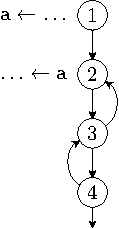
\includegraphics{liveness_dataflow_a.pdf}
       \quad
       \tikzfigure{liveness_dataflow_CFG}
       \qquad
       \label{fig:liveness_dataflow:a}
     }
     \hfill
     \subfloat[Loop nesting forest]{
       \label{fig:liveness_dataflow:b}
       % 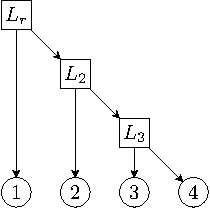
\includegraphics{liveness_dataflow_b.pdf}
       \tikzfigure{liveness_dataflow_LNF}
     }
     \hfill\null
   \end{center}
   \caption{Bad case for iterative data-flow analysis.}
   \label{fig:liveness_dataflow}
\end{figure}


\subsubsection{Correctness}
\label{sec:correctnessdebase}

%% The previous algorithms were specialized for the case where $\phi$-functions are interpreted as copies at the CFG edges preceding the $\phi$-functions.
%% For the correctness proofs, we resort to the following, more generic, $\phi$-semantics.
%% A $\phi$-function $a_0 = \phi(a_1, \ldots, a_n)$ at basic block~$B_0$, receiving its arguments from blocks $B_i$, $i>0$, is represented by a fresh variable $a_{\phi}$, a copy $a_0 = a_{\phi}$ at $B_0$, and copies $a_{\phi} = a_i$ at~$B_i$, for $i>0$.
%% Now, with respect to this $\phi$-function, $a_i$, for $i>0$, is not live-out at $B_i$ and $a_0$ is not live-in at $B_0$ anymore.
%% As for $a_{\phi}$, since it is not an SSA variable, it is not covered by the following lemmas.
%% But its live-range is easily identified:
%% it is live-in at~$B_0$ and live-out at $B_i$, $i>0$, and nowhere else.
%% Other $\phi$-semantics extend the live-ranges of the $\phi$-operands with parts of the live-range of $a_{\phi}$ and can thus be handled by locally refining the live-in and live-out sets.
%% This explains why, in Algorithm~\ref{alg:dag_dfs}, $\PhiUses(B)$ is added to $\LiveOut(B)$ (Line~\ref{alg:dag_dfs:phi_use}), $\PhiKill(B)$ is added to $\LiveIn(B)$ (Line~\ref{alg:dag_dfs:phi_kill_union}), and $\PhiKill(S)$ is removed from $\LiveIn(S)$ (Line~\ref{alg:dag_dfs:phi_kill_minus}).
%% This ensures that the variable defined by a $\phi$-function is marked as live-in and its uses as live-out at the predecessors.
%% A similar adjustment appears on Line~\ref{alg:loop_dfs:phi_kill_minus} of Algorithm~\ref{alg:loop_dfs}.


The first pass propagates the liveness sets using a post-order traversal of the 
forward CFG, $\mathcal{F}_\mathcal{L}(G)$, obtained by removing all back-edges 
from the \@CFG $G$.
The first two lemmas show that this pass correctly propagates liveness information to the loop-headers of the original \@CFG.
\begin{lemma}
	\label{lemma:firstpass}
	Let~$G$ be a reducible CFG, $\var{v}$ an SSA variable, and~$d$ its definition.
        If~$L$ is a maximal loop not containing~$d$, then~$\var{v}$ is live-in 
        at the loop-header~$h$ of~$L$ iff there is a path in 
        $\mathcal{F}_\mathcal{L}(G)$ (i.e., back-edge free) from~$h$ to a use 
        of $\var{v}$ that does not go through $d$.
\end{lemma}

\begin{lemma}
	\label{lemma:firstpass2}
	Let~$G$ be a reducible CFG, $\var{v}$ an SSA variable, and~$d$ its definition.
	Let~$p$ be a node of~$G$ such that all loops containing~$p$ also contain~$d$.
        Then $\var{v}$ is live-in at~$p$ iff there is a path in 
        $\mathcal{F}_\mathcal{L}(G)$, from~$p$ to a use of $\var{v}$ that does 
        not go through $d$.
\end{lemma}

Pointers to formal proofs are provided in the last section of this chapter.
The important property used in the proof is the dominance property that enforces the full live-range of a variable to be dominated by its definition $d$.
As a consequence, any back-edge part of the live-range is dominated by $d$, and 
the associated loop cannot contain $d$.

Algorithm~\ref{alg:dag_dfs}, which propagates liveness information along the DAG $\mathcal{F}_\mathcal{L}(G)$, can only mark variables as live-in that are indeed live-in.
Furthermore, if, after this propagation, a variable~$\var{v}$ is missing in the live-in set of a CFG node~$p$, Lemma~\ref{lemma:firstpass2} shows that~$p$ belongs to a loop that does not contain the definition of~$\var{v}$.
Let~$L$ be such a maximal loop.
According to Lemma~\ref{lemma:firstpass}, $\var{v}$ is correctly marked as live-in at the header of~$L$.
The next lemma shows that the second pass of the algorithm (Algorithm~\ref{alg:loop_dfs}) correctly adds variables to the live-in and live-out sets where they are missing.
% Thus,
% if a variable $\var{v}$ is missing in the live-in set of~$p$, $p$ belongs to a
% loop which does not contain the definition of $\var{v}$ and whose header~$h$ is
% not~$p$. The next lemma concludes this analysis.

\begin{lemma}
	\label{lemma:secondpass}
	Let~$G$ be a reducible CFG, $L$ a loop, and $\var{v}$ an SSA variable.
	If $\var{v}$ is live-in at the loop-header of~$L$, it is live-in and live-out at every CFG node in~$L$.
\end{lemma}

The intuition is straightforward: a loop is a strongly connected component, and because $d$ is live-in of $L$, $d$ cannot be part of $L$. 


 \subsection{Liveness Sets on Irreducible Flow Graphs}
\label{sec:irreducible}

The algorithms based on loops described above are only valid for reducible 
graphs.
We can derive an algorithm that works for irreducible graphs as well as 
follows:
transform the irreducible\index{irreducible} graph to a reducible 
graph\index{reducible CFG}, such that the liveness in both graphs is 
\emph{equivalent}.
First of all we would like to stress two points:
\begin{enumerate}
\item We do not impose the transformed graph to be \emph{semantically 
equivalent} to the original one, only isomorphism of liveness is required.  
\item We do not actually modify the graph in practice, but 
  Algorithm~\ref{alg:dag_dfs} can be changed to simulate the modification of 
  some edges on the fly.
\end{enumerate}

There exists loop nesting forest representations with possibly multiple headers 
per irreducible loop.
For the sake of clarity (and simplicity of implementation), we consider a representation where each loop has a unique entry node as header.
In this case, the transformation simply relies in redirecting any edge $s\rightarrow t$ arriving in the middle of a loop to the header of the outermost loop (if it exists) that contains $t$ but not $s$.
The example of Figure~\ref{fig:examplecfg} illustrates this transformation, with the modified edge highlighted.
Considering the associated loop nesting forest (with nodes $2$, $5$, and $8$ as loop headers), edge $9\rightarrow 6$ is redirected to node $5$.

Obviously the transformed code does not have the same semantics than the original one.
But, because a loop is a strongly connected component, dominance relationship is unchanged.
As an example, the immediate dominator of node $5$ is $3$, both in the original and transformed CFG.
For this reason, any variable live-in of loop $L_5$---thus live everywhere in the loop---will be live on any path from $3$ to the loop.
Redirecting an incoming edge to another node of the loop---in particular, the header---does not change this behavior.

\begin{figure}[t]
  \begin{center}
    % \hfill
    \subfloat[Irreducible CFG] {
      \label{fig:examplecfg:a}
      % 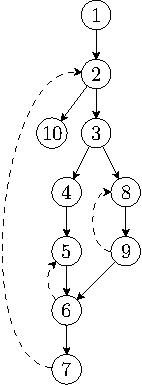
\includegraphics{examplecfg_a.pdf}
      % \quad
      \tikzsubfigure[1]{examplecfg}
      \quad
    }
    \hfill
    \subfloat[Reducible CFG] {
      % 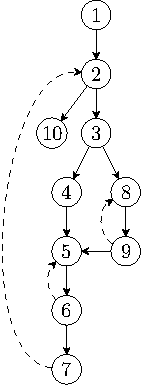
\includegraphics{examplecfg_c.pdf}
      % \quad
      \tikzsubfigure[2]{examplecfg}
      % \quad
      \label{fig:examplecfg:c}
    }
    \hfill
    \subfloat[Loop nesting forest]{
      \tikzfigure{exampleloop}
      \label{sub:examplecfgLNF}
    }
    % \hfill\strut
  \end{center}
  \caption{%
	  A reducible CFG derived from an irreducible CFG, using the loop nesting forest.
	  The transformation redirects edges arriving inside a loop to the loop header (here $9\rightarrow 6$ into $9\rightarrow 5$).}
  \label{fig:examplecfg}
\end{figure}

% \begin{figure}[t]
  % \begin{center}
    % 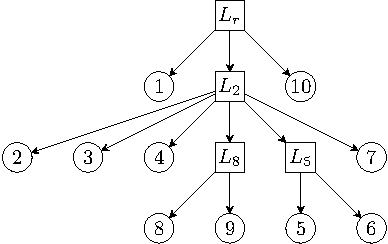
\includegraphics{exampleloop.pdf}
    % \tikzfigure{exampleloop}
  % \end{center}
  % \caption{A rooted loop-nested forest for the CFG of Figure~\ref{fig:examplecfg}.}
  % \label{fig:exampleloop}
% \end{figure}

\newcommand{\OLE}[2]{#1.\textit{OLE}\,(#2)}

To avoid building this transformed graph explicitly, an elegant alternative is to modify the CFG traversal in Algorithm~\ref{alg:dag_dfs}.
Whenever an entry-edge $s\rightarrow t$ is encountered during the traversal, instead of visiting $t$, we visit the header of the largest loop containing $t$ and not $s$.
This header node is nothing else than the highest ancestor of~$t$ in the loop nesting forest that is not an ancestor of~$s$.
We represent such as node as $\OLE{t}{s}$ (for ``Outermost Loop Excluding'').
As an example in Figure~\ref{fig:examplecfg},
considering edge $9\rightarrow 6$, the highest ancestor of $6$ not an ancestor of $9$ is $\OLE{9}{6}=L_5$. 
Overall, the transformation amounts to replacing all occurrences of~$S$ by $\OLE{S}{B}$ at Lines~\ref{alg:dag_dfs:irreducible_dfs} and~\ref{alg:dag_dfs:irreducible} of Algorithm~\ref{alg:dag_dfs}, which allows it to handle irreducible control-flow graphs.


\newcommand{\couple}[2]{\langle#1,#2\rangle}
\def\sep{,$ $}

\subsection{Computing the Outermost Excluding Loop (\textit{OLE})}
\label{sec:ole}
Our approach involves potentially many outermost excluding loop queries, especially for the liveness check algorithm as developed further.
An efficient implementation of \textit{OLE} is required.
The technique proposed here and shown in Algorithm~\ref{alg:hnca} is to pre-compute the set of ancestors from the loop-tree for every node.
A simple set operation can then find the node we are looking for:
the ancestors of the definition node are removed from the ancestors of the query point.
From the remaining ancestors, we pick the shallowest.
Using bitsets for encoding the set of ancestors of a given node, indexed with a topological order of the loop tree, this operations are easily implemented.
The removal is a bit inversion followed by a bitwise ``and'' operation, and the shallowest node is found by searching for the first set bit in the bitset.
Since the number of loops (and thus the number loop-headers) is rather small, the bitsets are themselves small as well and this optimization does not result in much wasted space.

Consider a topological indexing of loop-headers: $n.\textrm{LTindex}$ ($n$~being a loop-header) or reciprocally $i.\textrm{node}$ ($i$~being an index).
For each node, we associate a bitset (indexed by loop-headers) of all its ancestors in the loop tree:
$n.\textrm{ancestors}$.
This can be computed using any topological traversal of the loop-tree by a call of \textsc{DFS\_compute\_ancestors}($L_r$).
Notice that some compiler intermediate representations sometimes consider $L_r$ as a loop header.
Considering so in \textsc{DFS\_compute\_ancestors} will not spoil the behavior of \@\textit{OLE}.

\begin{algorithm}
  \Func{DFS\_compute\_ancestors(node~$n$)}{
    \uIf{$n \neq L_r$}{
      $n.\textrm{ancestors} \gets n.\textrm{LTparent.ancestors}$\;
    }
    \Else{
      $n.\textrm{ancestors} \gets \emptyset$\Comment*{empty bitset}
    }
    \If{$n.\textrm{isLoopHeader}$}{
      $n.\textrm{ancestors.add}(n.\textrm{LTindex})$
    }
    \ForEach{$s$ in $n.\textrm{LTchildren}$}{
      \textsc{DFS\_compute\_ancestors}($s$)
    }
  }
\caption{Compute the loop nesting forest ancestors.}
\label{alg:ancestors}
\end{algorithm}

Using this information, finding the outermost excluding loop can be done by simple bitset operations as in Algorithm~\ref{alg:hnca}.

\begin{algorithm}
  \Func{OLE(node \textit{self}, node~$b$)}{
    $\textit{nCA} \gets \textrm{bitset\_and}(\textit{self}.\textrm{ancestors}, \textrm{bitset\_not}(b.\textrm{ancestors}))$\;
    \uIf{$\textit{nCA}.\textrm{isempty}$}{
      \Return \textit{self}
    }\Else{
      \Return $\textit{nCA}.\textrm{bitset\_leading\_set.node}$\;
    }
  }
\caption{Outermost excluding loop.}
\label{alg:hnca}
\end{algorithm}

\begin{example}
	Consider the example of Figure~\ref{sub:examplecfgLNF} again and suppose the loops $L_2$, $L_8$, and $L_5$ are respectively indexed~$0$,$1$, and~$2$.
	Using big-endian notations for bitsets, Algorithm~\ref{alg:ancestors} would give labels $110$ to node $9$ and $101$ to node $6$.
	The outermost loop containing~$6$ but not~$9$ is given by the leading bit of $101\wedge \lnot 110=001$, \ie $L_5$.
\end{example}



\section{Liveness Check using Loop Nesting Forest and \Reduced\ Reachability}
\label{sec:live-check}


In contrast to liveness sets, liveness check\index{liveness check} does not provide the set of variables live at a block, but provides a query system to answer questions such as ``is variable $v$ live at location $q$?''
Such a framework is well suited for tree-scan based register allocation, SSA destruction, or Hyperblock scheduling.
Most register-pressure aware algorithms such as code-motion are not designed to take advantage of liveness a check query system and still require sets.
Such a query system can obviously be built on top of pre-computed liveness sets.
Queries in $O(1)$ are possible, at least for basic block boundaries, providing the use of sparsesets or bitsets to allow for efficient element-wise queries.
If sets are only stored at basic block boundaries, to allow a query system at instruction granularity, it is possible to use the list of uses of variables or backward scans.
Constant time worst case complexity is lost in this scenario and liveness sets that have to be incrementally updated at each (even minor) code transformation can be avoided and replaced by less memory consuming data structures that only depend on the \@CFG.

In the following, we consider the live-in query of variable $\var{a}$ at node $q$.
To avoid notational overhead, let $\var{a}$ be defined in the CFG node $d=\ldef{a}$ and let $u \in \luse{a}$ be a node where $\var{a}$ is used.
Suppose that $q$ is strictly dominated by $d$ (otherwise $v$ cannot be live at $q$).
Lemmas~\ref{lemma:firstpass}, \ref{lemma:firstpass2}, and~\ref{lemma:secondpass} stated in Section~\ref{sec:correctnessdebase} can be rephrased as follow:
\begin{enumerate}
\item
	Let $h$ be the header of the maximal loop containing $q$ but not $d$.
	Let $h$ be $q$ if such maximal loop does not exist.
	Then $v$ is live-in at $h$ if and only if there exists a forward path that goes from $h$ to $u$.
\item
	If $v$ is live-in at the header of a loop then it is live at any node inside the loop.
\end{enumerate}

In other words, $v$ is live-in at $q$ if and only if there exists a forward path from $h$ to $u$ where $h$ is, if it exists, the header of the maximal loop containing $q$ but not $d$, and $q$ itself otherwise.
Given the forward control-flow graph and the loop nesting forest, finding out if a variable is live at some program point can be done in two steps.
First, if there exists a loop containing the program point $q$ and not the definition, pick the header of the biggest such loop instead as the query point.
Then check for reachability from $q$ to any use of the variable in the forward \@CFG.
As explained in Section~\ref{sec:irreducible}, for irreducible CFG, the \emph{modified forward CFG} that redirects any edge $s\rightarrow t$ to the loop header of the outermost loop containing $t$ but excluding $s$ ($\OLE{t}{s}$), has to be used instead.
Correctness is proved from the theorems used for liveness sets.

\newcommand{\BB}[1]{\textrm{basicBlock}(#1)}
\newcommand{\ordering}[1]{\textrm{order}(#1)}
\newcommand{\isLoopHeader}[1]{\textrm{isLoopHeader}(#1)}
\newcommand{\FR}[2]{\textrm{{\reduced}Reachable}(#1,#2)}

Algorithm~\ref{alg:liveinchk} puts a little bit more efforts onto the table to provide a query system at instructions granularity.
If $q$ is in the same basic block than $d$ (lines~8-13), then $v$ is live at $q$ if and only if there is a use outside the basic block, or inside but after $q$.
If $h$ is a loop-header then $v$ is live at $q$ if and only if a use is forward reachable from $h$ (lines~19-20).
Otherwise, if the use is in the same basic block than $q$ it must be after $q$ to bring the variable live at $q$ (lines 17-18).
In this pseudo-code, upper cases are used for basic blocks while lower case are used for program points at instructions granularity.
``def($a$)'' is an operand.
``uses($a$)'' is a set of operands.
``\BB{$u$}'' returns the basic block containing the operand $u$.
Given the semantics of the \phifun instruction, the basic block returned by this function for a \phifun operand can be different from the block where the instruction textually occurs.
Also, ``$u$.order'' provides the corresponding (increasing) ordering in the basic block.
For a \phifun\ operand, the ordering number might be greater than the maximum ordering of the basic block if the semantics of the \phifun\ places the uses on outgoing edges of the predecessor block.
$\OLE{Q}{D}$\ corresponds to Algorithm~\ref{alg:hnca} given in Section~\ref{sec:ole}.
$\FR{H}{U}$, which tells if $U$ is reachable in the modified forward CFG, will be described later.

\begin{algorithm}
  \Func{IsLiveIn(programPoint $q$, var $\var{a}$)}{
    $d \gets \ldef{a}$\;
    $D \gets \BB{d}$\;
    $Q \gets \BB{q}$\;
    \If{$\textrm{not} \left(\strut D \sdom Q \textrm{ or } (D = Q \textrm{ and } \ordering{d} < \ordering{q})\right)$}{
      \Return $\textit{false}$\;
    }
    \If{$Q = D$}{
      \ForEach{$u \textbf{ in } \luse{\var{a}}$}{
        $U\gets \BB{u}$\;
        \If{$U \neq D \textrm{ or } \ordering{q} \leq \ordering{u}$}{
	  \Return $\textit{true}$\;
        }
      }
      \Return $\textit{false}$\;
    }
    $H \gets \OLE{Q}{D}$\;
    \ForEach{$u \textbf{ in } \luse{\var{a}}$}{
      $U\gets \BB{u}$\;
      \If{$\left(\textrm{not }\isLoopHeader{H}\right) \textrm{ and } U = Q  \textrm{ and } \ordering{u} < \ordering{q}$}{
        $\textbf{continue}$\;
      }
      \If{$\FR{H}{U}$}{
        \Return $\textit{true}$\;
      }
    }
    \Return $\textit{false}$\;
  }
\caption{Live-In Check.}
\label{alg:liveinchk}
\end{algorithm}

The live-out check algorithm, given by Algorithm~\ref{alg:liveoutchk} only differs from Live-in check in lines~5, 11, and~17 that involve ordering comparisons.
In line~5, if $q$ is equal to $d$ it cannot be live-in while it might be live-out; in lines~11 and~17 if $q$ is at a use point it makes it live-in but not necessarily live-out.

\begin{algorithm}
  \Func{IsLiveOut(programPoint $q$, var $\var{a}$)}{
     $d \gets \ldef{\var{a}}$\;
     $D \gets \BB{d}$\;
     $Q \gets \BB{q}$\;
    \If{$\textrm{not} \left(\strut D \sdom Q \textrm{ or } (D = Q \textrm{ and } \ordering{d} \leq \ordering{q})\right)$}{
       \Return $\textit{false}$ \Comment*{q must be dominated by the definition}
    }
    \If{$Q = D$}{
      \ForEach{$u \textbf{ in } \luse{\var{a}}$}{
         $U\gets \BB{u}$\;
	\If{$U \neq D \textrm{ or } \ordering{q} < \ordering{u}$}{
	   \Return $\textit{true}$\;
	}
      }
       \Return $\textit{false}$\;
    }
     $H \gets \OLE{Q}{D}$\;
    \ForEach{$u \textbf{ in } \luse{\var{a}}$}{
       $U\gets \BB{u}$\;
      \If{$\left(\textrm{not } \isLoopHeader{H}\right) \textrm{ and } U = Q  \textrm{ and } \ordering{u} \leq \ordering{q}$}{
	 $\textbf{continue}$\;
      }
      \If{$\FR{H}{U}$}{
	\Return $\textit{true}$
      }
    }
     \Return $\textit{false}$\;
  }
  \caption{Live-Out Check.}
  \label{alg:liveoutchk}
\end{algorithm}


\subsection{Computing the modified-\reduced\ reachability}

The liveness check query system relies on pre-computations for efficient \textit{OLE} and \textrm{{\reduced}Reachable} queries.
The outermost excluding loop is identical to the one used for liveness set.
We explain how to compute the modified-\reduced\ reachability here (i.e., 
forward-reachability on transformed CFG to handle irreducibility).
In practice we do not build explicitly the modified-\reduced\ graph.
To compute efficiently the modified-\reduced\ reachability we simply need to traverse the modified-\reduced\ graph in a reverse topological order.
A post-order initiated by a call to the recursive function \textrm{DFS\_Compute\_{\reduced}Reachable}($r$) (Algorithm~\ref{alg:computeFR}) will do the job.
Bitsets can be used to efficiently implement sets of basic blocks.
Once forward reachability have been pre-computed this way, $\FR{H}{U}$ returns true if and only if $U\in H\!.\textrm{{\reduced}Reachable}$.

\begin{algorithm}
  \Func{DFS\_Compute\_{\reduced}Reachable(block $N$)}{
     $N.\textrm{{\reduced}Reachable} \gets \emptyset$\;
     $N.\textrm{{\reduced}Reachable.add}(N)$\;
    \ForEach{$S\in \textrm{succs}(N)$ \textbf{if} $(N,S)$ is not a back-edge}{
       $H \gets \OLE{S}{N}$\;
       \If{$H.\textrm{{\reduced}Reachable} = \bot$}{\textrm{DFS\_Compute\_{\reduced}Reachable}$(H)$}
       $N.\textrm{{\reduced}Reachable} \gets  N.\textrm{{\reduced}Reachable} \cup H.\textrm{{\reduced}Reachable}$\;
    }
  }
\caption{Computation of modified-forward reachability using a traversal along a reverse topological order.}
\label{alg:computeFR}
\end{algorithm}

\section{Liveness Sets using Path Exploration}
\label{sec:path-explore}

Another maybe more intuitive way of calculating liveness sets is closely related to the definition of the live-range of a given variable.
As recalled earlier, a variable is live at a program point $p$, if $p$ belongs to a path of the CFG leading from a definition of that variable to one of its uses without passing through the definition.
Therefore, the live-range of a variable can be computed using a backward traversal starting at its uses and stopping when reaching its (unique) definition.

Actual implementation of this  idea could be done in several ways.
In particular the order along which use operands are processed, in addition to the way liveness sets are represented, can substantially impact the performance.
The one we choose the develop here allows to use a simple stack-like set representation so as to avoid any expensive set-insertion operations and set-membership tests.
The idea is simply to process use operands variable per variable.
In other words the processing of different variables is not intermixed, \ie the processing of one variable is completed before the processing of another variable begins.

Depending on the particular compiler framework, a preprocessing step that performs a full traversal of the program (\ie the instructions) might be required in order to derive the def-use chains\index{def-use chains} for all variables, \ie a list of all uses for each SSA-variable.
The traversal of the variable list and processing of its uses thanks to def-use chains is depicted in Algorithm~\ref{alg:var_by_var}.

Note that, in strict SSA form, in a given block, no use can appear before a definition.
Thus, if $\var{v}$ is live-out or used in a block~$B$, it is live-in iff it is not defined in~$B$.
This leads to the code of Algorithm~\ref{alg:up_and_mark_stack} for path exploration.


\begin{algorithm}[h]
    \Func{Compute\_LiveSets\_SSA\_ByVar(CFG)}{
      \ForEach{variable~$v$}{
        \ForEach{block~$B$ where~$v$ is used}{
          \If(\Comment*[f]{Used in the $\phi$ of a successor block}){$v \in \PhiUses(B)$}{
              $\LiveOut(B)=\LiveOut(B)\union\{v\}$
            }
            \textrm{Up\_and\_Mark}($B,v$)\;
        }
      }
    }
  \caption{Compute liveness sets per variable using def-use chains.}
  \label{alg:var_by_var}
\end{algorithm}




\begin{algorithm}[h]
    \Func{Up\_and\_Mark\_Stack($B,v$)}{
      \lIf{$\Def(v)\in B$ ($\phi$ excluded)}{
        \Return \Comment*[f]{Killed in the block, stop}
      }
      \lIf{$\top(\LiveIn(B)) = v$}{
        \Return \Comment*[f]{Propagation already done, stop}
      }
      $\push(\LiveIn(B), v)$\;
     \lIf{$v\in\PhiKill(B)$}{
       \Return \Comment*[f]{Do not propagate $\phi$ definitions}
     }
     \ForEach(\Comment*[f]{Propagate backwards}){$P\in\textrm{CFG\_preds}(B)$}{
       \If{$\top(\LiveOut(P)) \neq v$}{
         $\push(\LiveOut(P),v)$
       }
       \textrm{Up\_and\_Mark\_Stack}($P,v$)\;
      }
    }
  \caption{Optimized path exploration using a stack-like data structure.}
  \label{alg:up_and_mark_stack}
\end{algorithm}




\section{Further readings}
\label{sec:liveness:further}
Liveness information is usually computed with iterative
data-flow analysis, which goes back to Kildall~\cite{Kildall}. The algorithms are,
however, not specialized to the computation of liveness sets and overhead may
incur. Several strategies are possible, leading to
different worst-case complexities and performance in practice. Round-robin algorithms
propagate information according to a fixed block ordering derived from a
depth-first spanning tree and iterate until it stabilizes.  The complexity of
this scheme was analyzed by Kam et al.~\cite{novillo:bib:KU76}.  
Node listing algorithms specifies, a priori, the overall sequence of nodes, where repetitions are allowed, along which data-flow equations are applied.
Kennedy~\cite{Kennedy75} devises for structured flow graphs, node listings of size $2|V|$, with $|V|$ the number of control-flow nodes, and mentions the existence of node listings of size $O\left(|V| \log(|V|)\right)$ for reducible flow graphs.
Worklist algorithms focus on blocks that may need
to be updated because the liveness sets of their successors (for
backward problems) changed.
Empirical results by Cooper et al.~\cite{CHK06} indicate that the order in
which basic blocks are processed is critical and directly impacts the number of
iterations. They showed that, in practice, a mixed solution called ``single
stack worklist'' and based on a worklist initialized with a round-robin order is
the most efficient one  for liveness analysis. 

Alternative ways to solve data-flow problems belong to the family of elimina\-tion-based algorithms~\cite{RyPa86b}. Through recursive reductions of the 
CFG, variables of the data-flow system are successively eliminated and equations are reduced until the CFG reduces to a single node. 
The best, but unpractical, worst case complexity elimination algorithm has an almost-linear complexity $O(|E|\alpha(|E|))$. 
It requires the CFG (resp. the reverse CFG) to be reducible for a forward (resp.  backward) analysis.
For non-reducible flow-graphs, none of the existing approa\-ches can guarantee a worst case complexity better than $O(|E|^3)$.
In practice, irreducible CFGs are rare, but liveness
analysis is a backward data-flow problem, which frequently leads to
irreducible reverse CFGs. 

Gerlek et al.~\cite{gerlek94reference} use so-called $\lambda$-operators to collect upward exposed uses at control-flow split points.
Precisely, the $\lambda$-operators are placed at the iterated dominance frontiers, computed on the reverse CFG, of the set of uses of a variable.
These $\lambda$-operators and the other uses of variables are chained together and liveness is efficiently computed on this graph representation.
The technique of Gerlek et al.~can be considered as a precursor of the live variable analysis based on the Static Single Information (SSI) form conjectured by Singer~\cite{novillo:bib:S05} and revisited by Boissinot et al.~\cite{BoissinotBDR12}.
In both cases, insertion of pseudo-instructions guarantee that any definition is post-dominated by a use.

Another approach to compute liveness was proposed by
Appel~\cite[p.~429]{appel:2002:modern}. Instead of computing the liveness
information for all variables at the same time, variables are handled
individually by exploring paths in the CFG starting from variable uses. 
Using logic programming, McAllester~\cite{M02} presented an equivalent approach to show that liveness analysis can be performed in time
proportional to the number of instructions and variables.
However, his theoretical analysis is limited to a restricted input language
with simple conditional branches and instructions.
A more generalized analysis is given in Chapter~2 of the habilitation thesis of Rastello~\cite{rastello-hab}, both in terms of theoretical complexity and of practical evaluation (Section~\ref{sec:path-explore} describes path-exploration technique restricted to SSA programs).

The loop nesting forest considered in this chapter corresponds to the one obtained using Havlak's algorithm~\cite{Havlak:1997:TOPLAS}.
A more generalized definition exists and correspond to the \emph{minimal} loop nesting forest as defined by Ramalingam~\cite{Ramalingam:2002:TOPLAS}.
The handling of any minimal loop nesting forest is also detailed in Chapter~2 of\cite{rastello-hab}.

Handling of irreducible CFG can be done through CFG transformations such as node splitting~\cite{JC97,aho86compilers}.
Such a transformation can lead to an exponential growth in the number of nodes.
Ramalingam~\cite{Ramalingam:2002:TOPLAS} proposed a transformation (different than ours but also without any exponential growth) that only maintains dominance property (not the full semantic).

Finding the maximal loop not containing a node~$s$ but containing a node~$t$ (\textit{OLE}) is a problem similar to finding the least common ancestor\index{least common ancestor} (LCA) of the two nodes~$s$ and~$t$ in the rooted loop-nested forest:
the loop in question is the only direct child of $\textrm{LCA}(s,t)$, ancestor of~$t$.
As described in~\cite{BenderFC00}, an LCA query can be reduced to a Range Minimum Query (RMQ) problem that can itself be answered in $O(1)$, with a pre-computation of $O(n)$.
Adaptation of LCA to provide an efficient algorithm for \textit{OLE} queries is detailed in Chapter~2 of~\cite{rastello-hab}.

This Chapter is a short version of Chapter~2 of~\cite{rastello-hab} that among other details contains formal proofs and handling of different \phifun semantics. Sparsesets are described by Cooper and Torczon~\cite{cooper:2004:engineering}.

